\documentclass[a4paper,12pt]{report}

%Русский язык
\usepackage[T2A]{fontenc}
\usepackage[utf8]{inputenc}
\usepackage[english,russian]{babel}
\usepackage{cmap}

%Работа с кодом
\usepackage{listings}
\usepackage{color}

\definecolor{green}{rgb}{0,0.6,0}
\definecolor{gray}{rgb}{0.5,0.5,0.5}
\definecolor{red}{rgb}{0.6,0,0}

\lstset{
        language=Python, 
        basicstyle=\small\ttfamily, 
        numberstyle=\tiny,           
        columns=flexible,
        stepnumber=1,                   
        numbersep=5pt,        
        showspaces=false,
        showstringspaces=false,
        showtabs=false,
        tabsize=2,                
        captionpos=b,              
        breaklines=true,           
        breakatwhitespace=false,
        keywordstyle=\color{green},
        commentstyle=\color{gray},
        stringstyle=\color{red},      
}

%Математика
\usepackage{amsmath,amsfonts,amssymb,amsthm,mathtools} 

%Изображения
\usepackage{float}
\usepackage{graphicx}
\graphicspath{ {./img/} }

%Поля страницы
\usepackage{geometry} 
\geometry{left=2.3cm} 
\geometry{right=1.8cm} 
\geometry{top=2cm} 
\geometry{bottom=2.5cm} 

%Отступы
\usepackage{indentfirst}
\setlength{\parskip}{0cm}

\begin{document} 

\begin{titlepage}
\newpage
	\begin{center}
		\large Санкт-Петербургский политехнический университет Петра Великого\\
		Институт компьютерных наук и технологий\\
		Высшая школа интеллектуальных систем и суперкомпьютерных технологий\\
	\end{center}
\vspace{7cm}

\begin{center}
		\large \textbf{Отчёт по лабораторной работе №8} \\
		\textbf{Дисциплина:} Телекоммуникационные технологии\\
		\textbf{Тема:} Фильтрация и свёртка
\end{center}
\vspace{4cm}
	
\begin{flushright}
		\large Работу выполнил:\\ Ляшенко В.В.\\
		Группа: 3530901/80201\\
		Преподаватель:\\ Богач Н.В.
\end{flushright}

\vspace{\fill}
\begin{center}
	\large Санкт-Петербург\\ 2021
	\end{center}
\end{titlepage}

\tableofcontents
\listoffigures
\lstlistoflistings

\chapter{Упражнение 8.1}
    В начале мы запустим примеры из \texttt{chap08.ipynb}.
    
    В данном коде есть интерактивный виджет, в котором можно поэксперементировать с параметрами Гауссова окна и изучить их влияние на частоту среза. Воспользуемся им.
    
    Установим значение M = 20, std = 2 (Рис.1.1).
\begin{figure}[H]
        \centering
        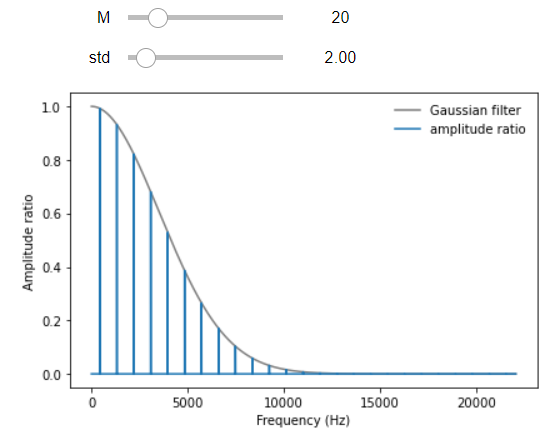
\includegraphics[width=0.8\textwidth]{fig1-1.PNG}
        \caption{Гауссово окно. std = 2}
        \label{fig:fig1-1}
\end{figure} 
    
    Теперь увеличим std до 3.5 (Рис.1.2).
\begin{figure}[H]
        \centering
        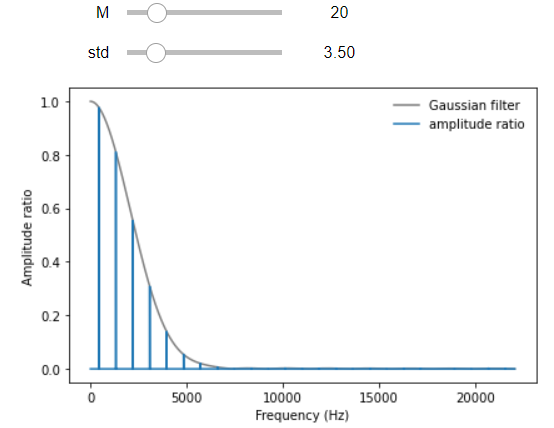
\includegraphics[width=0.8\textwidth]{fig1-2.PNG}
        \caption{Гауссово окно. std = 3.5}
        \label{fig:fig1-2}
\end{figure} 
    
    Продолжим увеличивать значение std до 6.5 (Рис.1.3).
\begin{figure}[H]
        \centering
        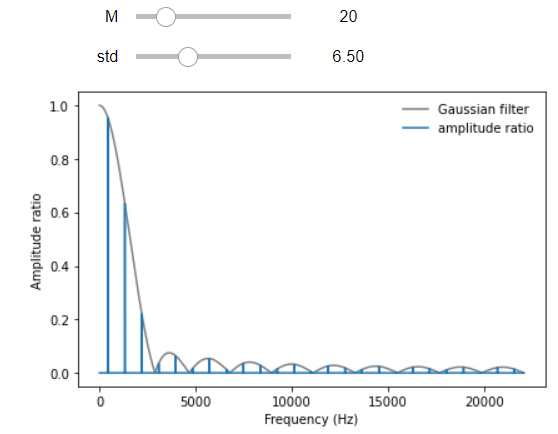
\includegraphics[width=0.8\textwidth]{fig1-3.PNG}
        \caption{Гауссово окно. std = 6.5}
        \label{fig:fig1-3}
\end{figure}  
    
    И, наконец, поставим максимальное значение std = 20 (Рис.1.4).
\begin{figure}[H]
        \centering
        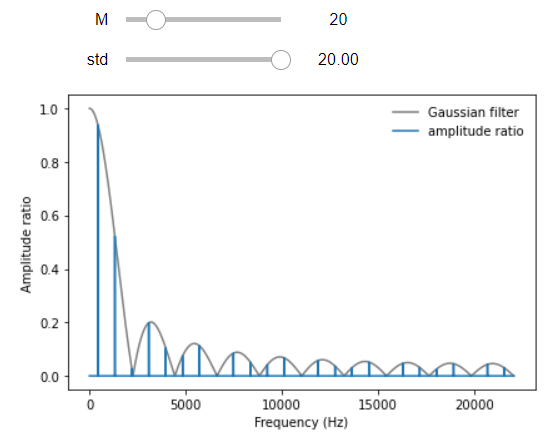
\includegraphics[width=0.8\textwidth]{fig1-4.PNG}
        \caption{Гауссово окно. std = 20}
        \label{fig:fig1-4}
\end{figure}

    Как мы можем видеть, без увеличения значения M, окно постепенно сжимается, высокочастотные гармоники в спектре спадают медленно и из-за этого появляются боковые лепестки. 
    
\chapter{Упражнение 8.2}
    Используем преобразование Фурье гауссовой кривой на нескольких примерах.
    
    Создадим функцию \texttt{plot\_gaussian}, которая создает окно Гаусса и его БПФ и отображает их графики. 
\begin{lstlisting}[caption=Функция plot\_gaussian]
       def plot_gaussian(std):
           M = 32
           gaussian = scipy.signal.gaussian(M=M, std=std)
           gaussian /= sum(gaussian)
    
           plt.subplot(1, 2, 1)
           plt.plot(gaussian)
           decorate(xlabel='Time')

           fft_gaussian = np.fft.fft(gaussian)
           fft_rolled = np.roll(fft_gaussian, M//2)
    
           plt.subplot(1, 2, 2)
           plt.plot(np.abs(fft_rolled))
           decorate(xlabel='Frequency')
           plt.show()

       plot_gaussian(2)
\end{lstlisting}    
\begin{figure}[H]
        \centering
        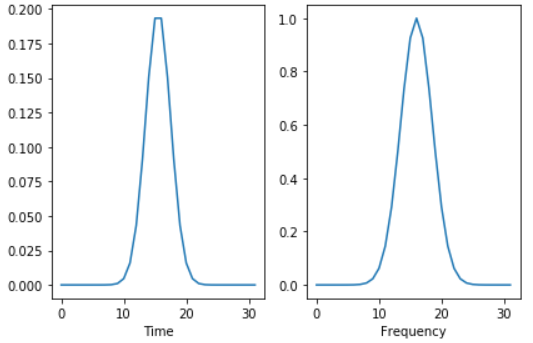
\includegraphics[width=0.8\textwidth]{fig2-1.PNG}
        \caption{Гауссово окно и его БПФ}
        \label{fig:fig2-1}
\end{figure}

    Теперь добавим слайдер, с помощью которого можно будет изменять std, и посмотрим, что происходит с ПФ.
    
\begin{figure}[H]
        \centering
        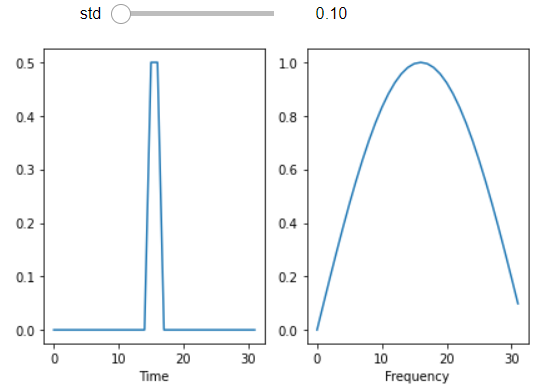
\includegraphics[width=0.8\textwidth]{fig2-2.PNG}
        \caption{Уменьшение std}
        \label{fig:fig2-2}
\end{figure}   
    При уменьшении std ПФ сжимается, а его БПФ расширяется (Рис.2.2).
    
\begin{figure}[H]
        \centering
        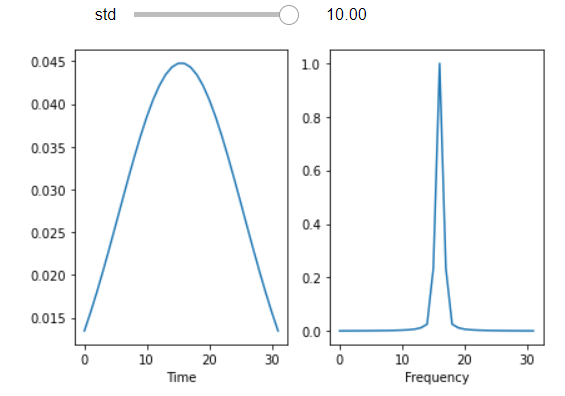
\includegraphics[width=0.8\textwidth]{fig2-3.PNG}
        \caption{Увеличение std}
        \label{fig:fig2-3}
\end{figure} 

    При увеличение мы видим обратную ситуацию, ПФ расширяется, а БПФ сужается.
    
    Таким образом, между ними есть обратная зависимость.
    
\chapter{Упражнение 8.3}
    Ранее мы изучали влияние на утечки спектра окна Хэмминга и некоторых других окон. Чтобы глубже понять эти окна, изучим их ДПФ.
    
    Создадим сигнал для дальнейшей работы с ним.
\begin{lstlisting}[caption=Создание сигнала]
       from thinkdsp import SquareSignal

       signal = SquareSignal(freq=440)
       wave = signal.make_wave(duration=1.0, framerate=44100)
\end{lstlisting}
    
    Затем построим все нужные нам окна и напечатем их графики. 
\begin{lstlisting}[caption=Построение окон]
       M = 15
       std = 2.5

       gaussian = scipy.signal.gaussian(M=M, std=std)   
       bartlett = np.bartlett(M)
       blackman = np.blackman(M)
       hamming = np.hamming(M)
       hanning = np.hanning(M)

       windows = [blackman, gaussian, hanning, hamming]
       names = ['blackman', 'gaussian', 'hanning', 'hamming']

       for window in windows:
           window /= sum(window)

       for window, name in zip(windows, names):
           plt.plot(window, label=name)

       decorate(xlabel='Index')
\end{lstlisting}    
\begin{figure}[H]
        \centering
        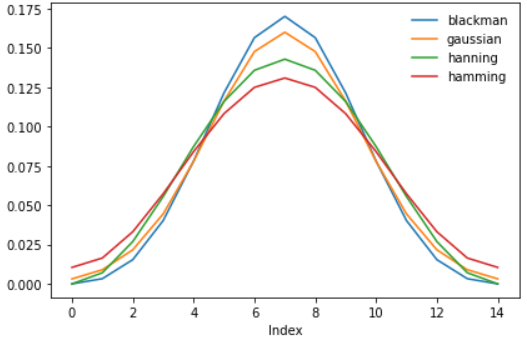
\includegraphics[width=0.8\textwidth]{fig3-1.PNG}
        \caption{Графики окон}
        \label{fig:fig3-1}
\end{figure}

     Как мы можем видеть на рис.3.1, их графики довольно похожи.

    Теперь получим их ДПФ.
\begin{lstlisting}[caption=Построение ДПФ]
       plot_window_dfts(windows, names)
       decorate(xlabel='Frequency (Hz)')
\end{lstlisting}
\begin{figure}[H]
        \centering
        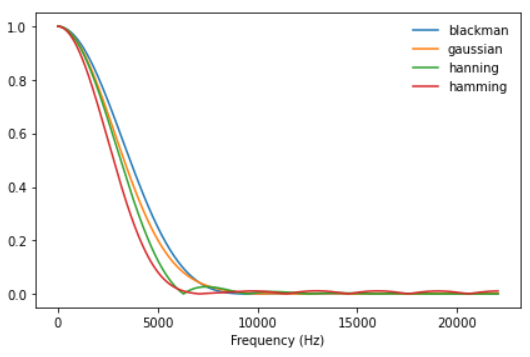
\includegraphics[width=0.8\textwidth]{fig3-2.PNG}
        \caption{ДПФ окон}
        \label{fig:fig3-2}
\end{figure}     
       
       Из рис.3.2 видно, что ДПФ окон тоже похожи. Однако Хэмминг спадает быстрее всех, Блэкман - медленнее всех, а у Ханнинга самые заметные боковые лепестки.
       
       Построим эти же графики в логарифмическом масштабе.
\begin{lstlisting}[caption=Построение ДПФ в логарифмическом масштабе]
       plot_window_dfts(windows, names)
       decorate(xlabel='Frequency (Hz)', yscale='log')
\end{lstlisting}
\begin{figure}[H]
        \centering
        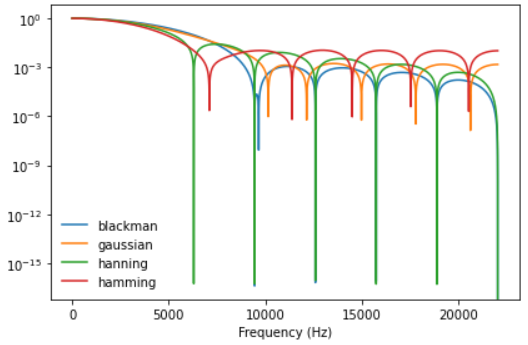
\includegraphics[width=0.8\textwidth]{fig3-3.PNG}
        \caption{ДПФ окон в логарифмическом масштабе}
        \label{fig:fig3-3}
\end{figure}  

    Из рис.3.3 мы можем увидеть, что сначала значения Хэмминга и Хеннинга падают быстрее, чем два других. Окна Гаусса и Хэмминга имеют самые стойкие боковые лепестки. Окно Ханнинга может иметь наилучшее сочетание быстрого падения и минимальных боковых лепестков.     
\chapter{Выводы}
    В результате выполнения данной работы мы изучили понятия фильтрации и свёртки. Также мы получили навыки работы с Гауссовым окном и лучше изучили разные окна, через их ДПФ.
\end{document}